% !TEX root = Séquence 2 - Activités - Vecteurs.tex
% Transcription des activités 2 (Découvrir les vecteurs) et 3 (Enchaîner
% deux translations) du manuel, en autonome (même montage que "Séquence 2 -
% Cours - Vecteurs.tex" : on recharge CLT2627.sty par \input direct à cause
% de l'espace dans le nom du dossier).
\documentclass[a4paper,11pt,french]{report}
\input{../TeX - Polycopié et Exercices/CLT2627.sty}
\graphicspath{{../TeX - Polycopié et Exercices/}}

\usetikzlibrary{shapes.misc, arrows.meta}
\tikzset{cross/.style={cross out, draw=black, minimum size=#1, inner sep=0pt}}

\begin{document}
\pagestyle{empty}
\fancypagestyle{plain}{\fancyhf{}\renewcommand{\headrulewidth}{0pt}\renewcommand{\footrulewidth}{0pt}}

% ----------------------------------------------------------------------
% Mise en forme "façon manuel" : pastille verte numérotée + titre + pastille
% durée, puis cadre vert englobant le contenu de l'activité. Ce sont des
% commandes locales à ce fichier (pas ajoutées à CLT2627.sty, qui est
% partagé avec le polycopié général).
% ----------------------------------------------------------------------
\definecolor{vertActivite}{RGB}{85,163,55}
\definecolor{orangePALP}{RGB}{224,120,40}

\newtcolorbox{ActiviteBox}{enhanced,breakable,colback=white,colframe=vertActivite,
  boxrule=1pt,arc=3pt,left=8pt,right=8pt,top=6pt,bottom=6pt}

\newtcolorbox{JauneBox}{enhanced,colback=yellow!12,colframe=yellow!55!black,
  boxrule=0.6pt,arc=2pt,left=6pt,right=6pt,top=4pt,bottom=4pt}

\newcommand{\Activite}[3]{%
\noindent
\begin{minipage}[c]{0.9cm}
\tikz\node[fill=vertActivite,text=white,font=\bfseries\Large,inner sep=0pt,
  minimum width=0.8cm,minimum height=0.8cm,rounded corners=3pt]{#1};
\end{minipage}%
\begin{minipage}[c]{0.68\linewidth}
{\bfseries\Large\color{vertActivite}#2}
\end{minipage}%
\begin{minipage}[c]{\dimexpr\linewidth-0.9cm-0.68\linewidth\relax}
\raggedleft\tikz\node[draw=gray,circle,inner sep=2.5pt,font=\scriptsize]{#3};
\end{minipage}

\smallskip
}

\newcommand{\PALP}{\tikz[baseline=-0.5ex]\node[draw=orangePALP,rounded corners=3pt,
  inner sep=3pt,font=\bfseries\small,color=orangePALP]{Pour aller plus loin};}

% Point représentant le palet : petit cercle avec une croix à l'intérieur.
\newcommand{\Palet}[1]{\node[draw,circle,inner sep=1.3pt] at #1 {\tiny$+$};}

\chapter*{Activités}
\vspace{-1.5em}

% ========================================================================
\Activite{2}{Découvrir les vecteurs}{10 min}
\begin{ActiviteBox}

Le jeu de hockey sur glace est un jeu d'équipe dont l'objectif est de marquer des points en amenant le palet dans le but à l'aide d'une crosse. Un joueur vient de glisser, amenant son palet du bout de la crosse. Voici un schéma du mouvement, qui indique que le joueur, la crosse et le palet ont subi le même déplacement. On observe que la main du joueur s'est déplacée du point Q au point Q'.

\begin{enumerate}
\item Quelle transformation reconnaît-on ?
\item
\begin{enumerate}
\item En quel point cette transformation transforme-t-elle le point A ?
\item En quel point cette transformation transforme-t-elle le point H ?
\end{enumerate}
\end{enumerate}

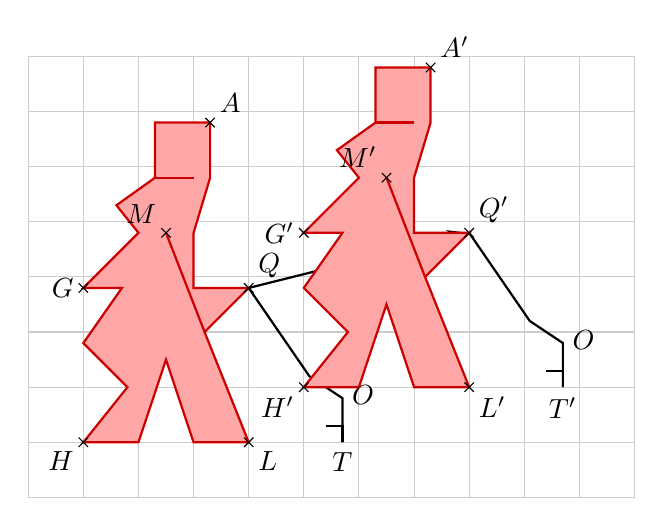
\begin{tikzpicture}[x=0.7cm, y=0.7cm]
    % Quadrillage de fond (11 colonnes, 8 lignes)
    \draw[step=1, gray!40, thin] (0,0) grid (11,8);

    % Style pour la couleur du bonhomme
    \tikzset{
        figure style/.style={fill=red!35, draw=red!80!black, thick}
    }

    % --- FIGURE INITIALE (à gauche) ---
    % Remplissage et contours de la figure
    \path[figure style] 
        (1,1) -- (2,1) -- (2.5,2.5) -- (3,1) -- (4,1) -- (3.2,3) -- (4,3.8) -- 
        (3,3.8) -- (3,4.8) -- (3.3,5.8) -- (3.3,6.8) -- (2.3,6.8) -- (2.3,5.8) -- (1.6,5.3) -- (2,4.8) -- 
        (1,3.8) -- (1.7,3.8) -- (1,2.8) -- (1.8,2) -- cycle;

    % Lignes intérieures du cou/épaule (gauche)
    \draw[red!80!black, thick] (2.3,5.8) -- (3,5.8);
    \draw[red!80!black, thick] (2.5,4.8) -- (3.2,3);

    % Points et étiquettes de la figure gauche
    \filldraw[black] (3.3,6.8) node[cross=3pt, rotate=0] {} node[above right] {$A$};
    \filldraw[black] (2.5,4.8) node[cross=3pt, rotate=0] {} node[above left] {$M$};
    \filldraw[black] (1,3.8) node[cross=3pt, rotate=0] {} node[left] {$G$};
    \filldraw[black] (1,1) node[cross=3pt, rotate=0] {} node[below left] {$H$};
    \filldraw[black] (4,1) node[cross=3pt, rotate=0] {} node[below right] {$L$};
    \filldraw[black] (4,3.8) node[cross=3pt, rotate=0] {} node[above right] {$Q$};

    % Ombre / Ligne d'appui O-T à gauche
    \draw[thick] (4,3.8) -- (5.1,2.2) -- (5.7,1.8) -- (5.7,1) node[below] {$T$};
    \draw[thick] (5.4,1.3) -- (5.7,1.3) -- (5.7,1);
    \node at (5.7,1.5) [above right] {$O$};


    % --- VECTOR DE TRANSLATION (v) ---
    \draw[-{Stealth[scale=1.2]}, thick] (4,3.8) -- (8,4.8) node[midway, above] {$\vec{v}$};


    % --- FIGURE TRANSLATÉE (à droite, décalée de (+4, +1)) ---
    \path[figure style] 
        (5,2) -- (6,2) -- (6.5,3.5) -- (7,2) -- (8,2) -- (7.2,4) -- (8,4.8) -- 
        (7,4.8) -- (7,5.8) -- (7.3,6.8) -- (7.3,7.8) -- (6.3,7.8) -- (6.3,6.8) -- (5.6,6.3) -- (6,5.8) -- 
        (5,4.8) -- (5.7,4.8) -- (5,3.8) -- (5.8,3) -- cycle;

    % Lignes intérieures du cou/épaule (droite)
    \draw[red!80!black, thick] (6.3,6.8) -- (7,6.8);
    \draw[red!80!black, thick] (6.5,5.8) -- (7.2,4);

    % Points et étiquettes de la figure droite
    \filldraw[black] (7.3,7.8) node[cross=3pt, rotate=0] {} node[above right] {$A'$};
    \filldraw[black] (6.5,5.8) node[cross=3pt, rotate=0] {} node[above left] {$M'$};
    \filldraw[black] (5,4.8) node[cross=3pt, rotate=0] {} node[left] {$G'$};
    \filldraw[black] (5,2) node[cross=3pt, rotate=0] {} node[below left] {$H'$};
    \filldraw[black] (8,2) node[cross=3pt, rotate=0] {} node[below right] {$L'$};
    \filldraw[black] (8,4.8) node[cross=3pt, rotate=0] {} node[above right] {$Q'$};

    % Ombre / Ligne d'appui O-T à droite
    \draw[thick] (8,4.8) -- (9.1,3.2) -- (9.7,2.8) -- (9.7,2) node[below] {$T'$};
    \draw[thick] (9.4,2.3) -- (9.7,2.3) -- (9.7,2);
    \node at (9.7,2.5) [above right] {$O$};

\end{tikzpicture}


\begin{JauneBox}
On dit qu'il s'agit de la \textbf{translation de vecteur} $\Vj{QQ'}$ ou $\Vj{AA'}$ ou $\Vj{HH'}$ et que les vecteurs $\Vj{QQ'}$, $\Vj{AA'}$ et $\Vj{HH'}$ sont \textbf{égaux}.
\end{JauneBox}

\begin{enumerate}
\setcounter{enumi}{2}
\item
\begin{enumerate}
\item Décrire des caractéristiques communes de ces vecteurs.
\item Quelle est la nature des quadrilatères QQ'A'A et QQ'H'H ? Justifier.
\end{enumerate}
\item
\begin{enumerate}
\item Quelle semble être la nature du quadrilatère AA'H'H ?
\item Les vecteurs $\Vj{AH}$ et $\Vj{A'H'}$ sont-ils égaux ? Citer d'autres couples de vecteurs égaux.
\end{enumerate}
\item \PALP\ Les points images de trois points alignés sont-ils aussi alignés ?
\end{enumerate}

\end{ActiviteBox}

\bigskip

% ========================================================================
\Activite{3}{Enchaîner deux translations}{20 min}
\begin{ActiviteBox}

On reprend le contexte du jeu de hockey de l'activité précédente. La patinoire est vue de dessus. Au cours du jeu, le palet va subir plusieurs déplacements représentés par les vecteurs dans la figure ci-contre.

\begin{enumerate}
\item
\begin{enumerate}
\item Reproduire la figure.
\item Construire l'image $A_1$ du palet $A$ par la translation de vecteur $\Vj{u}$.
\item Enchaîner par la construction de $A_2$ image de $A_1$ par la translation de vecteur $\Vj{w}$.
\item En admettant que l'enchaînement de ces deux translations est une translation, tracer le vecteur qui lui est associé.
\end{enumerate}
\end{enumerate}

\begin{center}
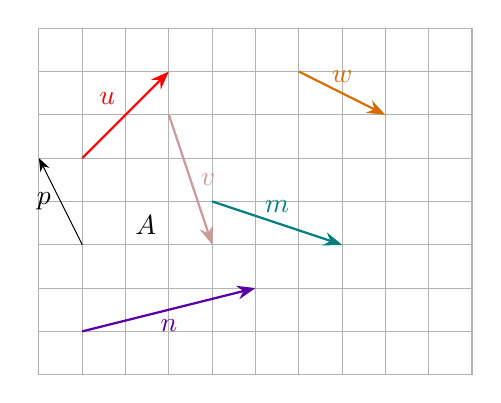
\begin{tikzpicture}[scale=0.55, >=Stealth]
\draw[thin,gray!60] (0,0) grid (10,8);
\Palet{(2,3)} \node[above right] at (2,3) {$A$};

\draw[->,thick,red] (1,5) -- (3,7) node[midway,above left]{$\Vj u$};
\draw[->,thick,orange!85!black] (6,7) -- (8,6) node[midway,above]{$\Vj w$};
\draw[->,thick,violet!70!blue] (1,1) -- (5,2) node[midway,below]{$\Vj n$};
\draw[->,thick,teal] (4,4) -- (7,3) node[midway,above]{$\Vj m$};
\draw[->,thick,pink!80!black] (3,6) -- (4,3) node[midway,right]{$\Vj v$};
\draw[->,thin,black] (1,3) -- (0,5) node[midway,left]{$\Vj p$};
\end{tikzpicture}
\end{center}

\begin{JauneBox}
L'enchaînement de ces deux translations correspond à la translation de vecteur $\Vj u+\Vj w$.
\end{JauneBox}

\begin{enumerate}
\setcounter{enumi}{4}
\item[e)] À quel vecteur de la figure est égal le vecteur $\Vj u+\Vj w$ ?\\
\textcolor{white}{Le vecteur $\Vj u+\Vj w$ est égal au vecteur $\Vj n$ de la figure.}
\end{enumerate}

\begin{enumerate}
\setcounter{enumi}{1}
\item
\begin{enumerate}
\item Le jeu continue : construire $A_3$ l'image de $A_2$ par la translation de vecteur $\Vj p$ puis $A_4$ l'image de $A_3$ par la translation de vecteur $\Vj v$.
\item Construire un vecteur qui correspond au vecteur $\Vj p+\Vj v$.
\end{enumerate}
\end{enumerate}

\bigskip

\PALP\quad Le but est marqué si le palet rentre dans le demi-cercle de diamètre [BC] de la figure ci-contre.

En subissant successivement les translations de vecteurs $\Vj r$, $\Vj s$, $\Vj t$ et $\Vj a$, le palet atteint-il le but ?

\begin{center}
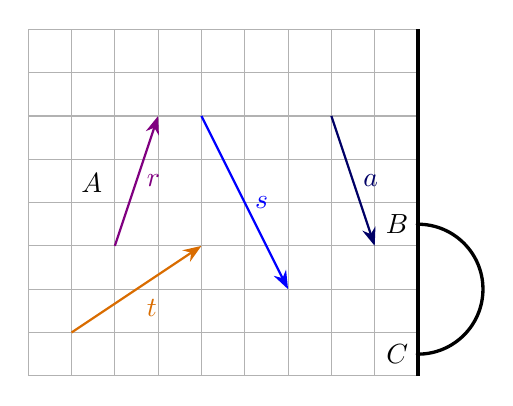
\begin{tikzpicture}[scale=0.55, >=Stealth]
\draw[thin,gray!60] (0,0) grid (9,8);
\draw[very thick] (9,0) -- (9,8);
\Palet{(1,4)} \node[above right] at (1,4) {$A$};

\draw[->,thick,violet] (2,3) -- (3,6) node[midway,right]{$\Vj r$};
\draw[->,thick,blue] (4,6) -- (6,2) node[midway,right]{$\Vj s$};
\draw[->,thick,orange!85!black] (1,1) -- (4,3) node[midway,below right]{$\Vj t$};
\draw[->,thick,blue!40!black] (7,6) -- (8,3) node[midway,right]{$\Vj a$};

\draw[very thick] (9,0.5) arc[start angle=-90,end angle=90,radius=1.5];
\fill (9,3.5) circle (1.5pt) node[left]{$B$};
\fill (9,0.5) circle (1.5pt) node[left]{$C$};
\end{tikzpicture}
\end{center}

\medskip
\textcolor{white}{En cumulant $\Vj r+\Vj s+\Vj t+\Vj a$, le palet arrive au point de coordonnées $(8;2)$ (en partant de $A(1;4)$), qui est bien à l'intérieur du demi-cercle de diamètre [BC] (centre $(9;2)$, rayon $1,5$) : le palet atteint donc le but.}

\end{ActiviteBox}

\end{document}
